\documentclass{llncs}

\usepackage{graphicx,float,wrapfig}
\usepackage{epstopdf}
\usepackage[style=base]{caption}
\usepackage{subcaption}
\captionsetup{compatibility=false}
%
%\title{Experimental Platform for Human Robot Interaction based on Human Motions}
\title{An intuitive interface for designing social behaviors based on human motions}
%
\titlerunning{ExPriMot}  % abbreviated title (for running head)
%                                     also used for the TOC unless
%                                     \toctitle is used
%
\author{Praveenkumar Vasudevan\inst{1} \and Gentiane Venture\inst{2}}
%
\authorrunning{Praveenkumar Vasudevan et al.} % abbreviated author list (for running head)
%\
%%%% list of authors for the TOC (use if author list has to be modified)
\tocauthor{Praveenkumar Vasudevan, Gentiane Venture}
%
\institute{Graduate Student, \'{E}cole Centrale de Nantes, Nantes, France,\\
\email{praveenv4k@gmail.com}
\and
Associate Professor, Tokyo University of Agriculture and Technology, Japan\\
\email{venture@cc.tuat.ac.jp}}
\begin{document}
\maketitle   
\begin{abstract}
	Humans interacting with intelligent robots has been seen as a potential game changer of the future. In scenarios where robots coexist with humans in a social environment, understanding not only verbal communication, but also non-verbal communication is extremely inevitable. The non-verbal communication carries information such as intention, emotion and health of a human, that adds value to the way robots participate in an interaction. Additionally, the people who design interaction scenarios are from diverse fields who do not essentially have the required robot programming skills. In this paper we propose an easy to use and intuitive programming interface which gives the power to design robot behaviors taking into account human motions. We propose a distributed architecture which gives the capability to plug and play multi-modal motion recognition systems and diverse class of robots. We present results of NAO humanoid robot performing actions understanding human motions using Kinect motion recognition system.
\keywords{human robot interaction, motion recognition, robot behaviors, kinect, nao}
\end{abstract}
\section{Introduction}
\quad The richness and diversity of Human Robot Interaction (HRI) has been described in \cite{dautenhahn2007methodology} as ``HRI is a challenging research field at the intersection of psychology, cognitive science, social sciences, artificial intelligence, computer science, robotics, engineering and human-computer interaction". Goodrich in his extensive survey \cite{goodrich2007human} proposed two main types of HRI namely remote interaction and proximate interaction. The latter is particularly important where the humans and the robots are co-located. Proximate interaction has gained importance due to the successful encounters of putting robots to work with human beings. It has led to the development of a new class of robots called social robots. Yan et al. \cite{yan2014survey} define ``A social robot is a robot which can execute designated tasks and the necessary condition turning a robot into a social robot is the ability to interact with humans by adhering to certain social cues and rules.''

	Social robots already entered the human spaces as entertainers, educators, caring agents and personal assistants \cite{Aldebaran}. Hence the design and the development of interaction systems need to be approached in a systematic manner wherein the robots should be able to understand the human motions and intentions in order to interact in a better way. To make it possible it is necessary to develop robotic systems with essential perceptual ability for efficient and natural interaction. Most often the on-board sensors on the robots fail to satisfy this demanding requirement due to various constraints like space, power and computational needs. Therefore consideration of augmenting exteroceptive sensors that are commonly available in the smart home/public environments to this purpose is essential.

	Another important aspect in HRI is the fact that the users of such systems are from diverse backgrounds. People study various aspects such as robot ethics, social acceptance, liveliness, cultural influence etc., from various perspectives like sociology, psychology, humanities and so on. So the tools needed to design behaviors of a social robot should be intuitive and user friendly.  With increased availability of social robots and cost effective motion recognition sensors, we could still observe a huge void which inhibits the exploitation of available technology for designing human motion driven robot behaviors.

	The main contribution of this work is to develop an application independent experimental platform wherein a social robot is augmented with essential perceptual ability to understand human motions. The behavior design of such a social robot is made possible by an easy to use behavior design interface. The resulting experimental platform could be used by people from interdisciplinary fields to design the interaction between social robots and humans. Although our behavior design framework could accommodate variety of robots and sensors, we present the scenarios targeted for the NAO \cite{NaoRobot} humanoid robot and commercially available Kinect \cite{Kinect2014} RGB-D camera for localization and gesture recognition. 
\section{Related work}
\quad Vision based motion capture and analysis systems have been one of the first class citizens in the human motion capture and analysis. It has been studied widely and a summary of all the approaches developed during the past decade has been presented in the surveys \cite{moeslund2006survey}\cite{poppe2007vision}. Vision based human pose estimation has traditionally suffered from the requirement to adopt an initialization pose and losing track after a few frames. These problems have been addressed by the approaches proposed by Xbox team \cite{Kinect2014} which are capable of accurately tracking human skeletons using single depth images \cite{shotton2013efficient}. Understanding of human motion is not complete if the action of the human could not be inferred. In the survey by Microsoft research team \cite{han2013enhanced}, a background study on various algorithms used for human activity analysis is presented. Recently data-driven machine learning approaches have proven to be successful with recognition accuracy as high as 94.9\% \cite{Kinect2014}.
	
	The localization of humanoid robots is a challenging issue, due to rough odometry estimation, noisy onboard sensing, and the swaying motion caused by walking \cite{cervera2012localization}. The Point cloud library \cite{rusu20113d}, one of the most widely used 3d perception library, implements ready to use probabilistic tracking algorithms. Studies on robot localization, obstacle mapping, and path planning by equipping NAO with a consumer-level depth camera have been reported in \cite{maier2012real}. Localization and motion planning in smart home environment using an external kinect sensor have been proposed in \cite{cervera2012localization}. These methods are computationally demanding and it could cause overall performance degradation particularly when one wants to share the same sensor for both human motion recognition and localization of the robot. Tracking rectangular fiducial markers using augmented reality tool-kits like ALVAR \cite{ALVAR} can be interesting if one could embed those markers on the humanoid robot. This is one of the simplest and cheapest solutions in terms of computational power as it can provide position and orientation of the physical markers in real time.
	
	The users of social robots do not have necessarily backgrounds in programming and design of robot behaviors. The main challenge in the behavior design is the ability to define the behavior which can abstract complex data flows from the end user. There exists flow-chart based visual programming languages \cite{NaoRobot} which allow non-programmers to create robot applications using a set of pre-built behavioral blocks. These programs are very intuitive but when it comes to designing reactive behaviors for human-in-the-loop scenarios, the existing visual programming methods increase the cognitive load on the end users. Specialized robot programming techniques like Task description language \cite{simmons1998task} and middlewares like ROS \cite{quigley2009ros} have been proposed in the literature. Though these systems provide modular and distributed architecture, support multiple sensors and robots etc., these require high level of skill in robotics and programming. Recently non-domain-specific solution like Targets-Drives-Means is proposed in \cite{berenz2014targets}, however it lacks an intuitive interface.
	
	Nowadays there has been a lot of efforts to teach programming to children and people without computer science background \cite{Scratch}\cite{Blockly}. These tools are very intuitive and have already been proven to be used by novice programmers to build games and educational applications. The Blockly library \cite{Blockly} from Google offers a complete client side JavaScript library which could be used for developing custom blocks and code generators as per the application requirements.
\section{Motion Driven Behavior Interface}
\quad We propose a light weight interface for designing human motion driven behaviors taking inspiration from distributed architecture \cite{quigley2009ros} and intuitive visual programming techniques \cite{Blockly}. 
\subsection{System Architecture}
The system setup and architecture are shown in Fig~\ref{fig:architecture}.
The principal components of the architecture are
\begin{figure}
\centering
\begin{subfigure}[t]{0.46\textwidth}
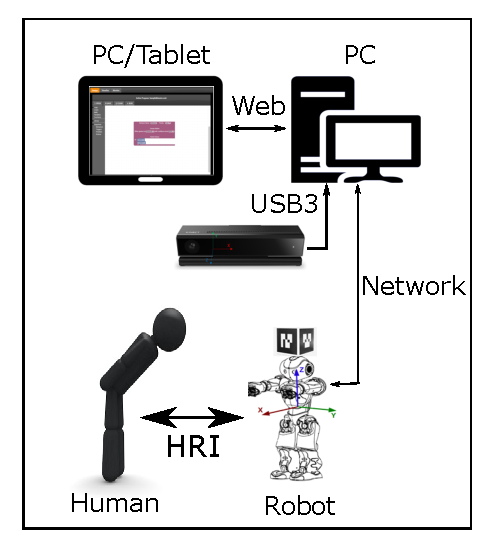
\includegraphics[width=\textwidth]{../thesis/assets/system_setup.eps}
\caption[System Setup]{System Setup}
\end{subfigure}
\begin{subfigure}[t]{0.48\textwidth}
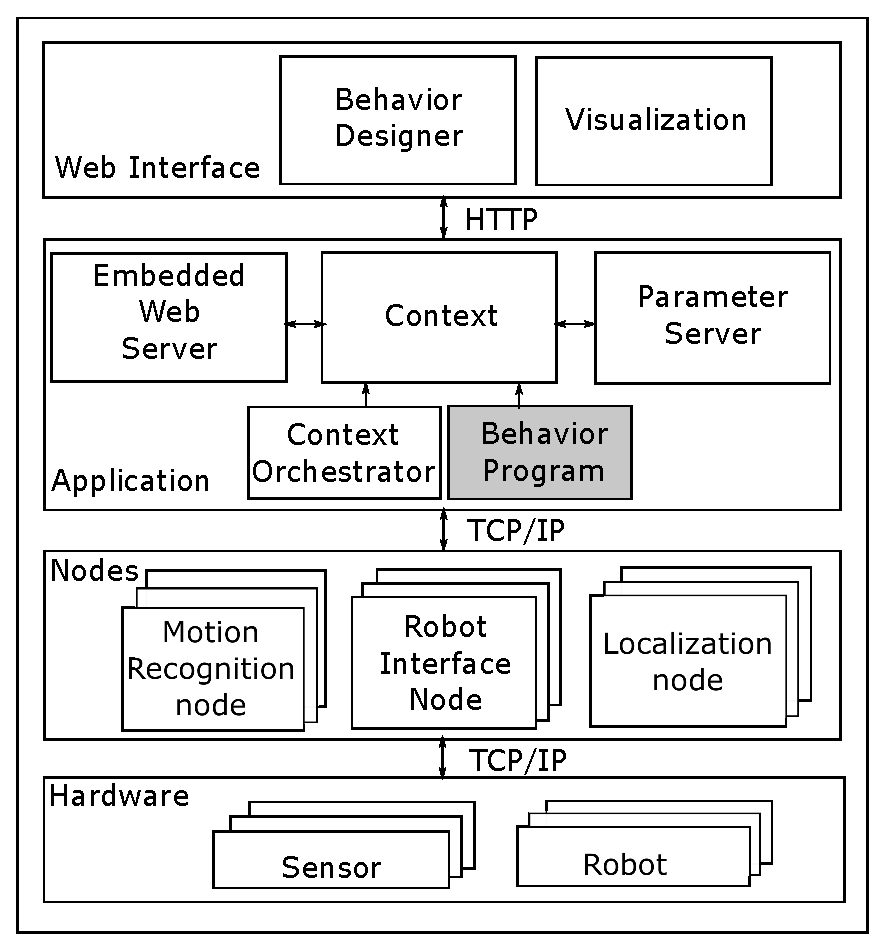
\includegraphics[width=\textwidth]{../thesis/assets/architecture.eps}
\caption[System Architecture]{Architecture}
\end{subfigure}
\caption[System Architecture]{Motion Driven behavior interface}
\label{fig:architecture}
\end{figure}
\begin{itemize}
\item \textbf{Application Components}
\begin{itemize}
\item \emph{Context}: The application context contains the complete description of the world. It contains latest information about all the robots including their location, sensor data, status etc., It also contains information about all the humans in the environment along with their active motions/gestures as supplied by the motion recognition modules.
\item \emph{Parameter Server}: The parameter server acts as a central repository for managing the parameters of the system and of the distributed components.
\item \emph{Embedded Web Server}: The web server embedded in the application serves the file and data requests from the web client.
\item \emph{Context Orchestrator}: The orchestrator keeps the Context uptodate by synchronizing with information of the robots and humans published by the distributed components.
\item \emph{Behavior Program} : A dynamic component that will be created when the user starts the program he/she designed using the user interface. The declarative description of the behavior described in Section~\ref{ssec:behavior_program} is parsed in order to create a memory model. The behavior program node monitors the application context for the motion triggers and invokes the corresponding robot actions according to the way it is being described in the program.
\end{itemize}
\item \textbf{Distributed Components} : These are nodes in the system each with a specific goal that can be started/stopped at any time during the entire application life-cycle without affecting the other nodes or the system. All the nodes will communicate with the application using message passing techniques. They can run in any machine inside the network.
\begin{itemize}
\item \emph{Motion Recognition Node} : A dedicated node that interacts with a motion recognition sensor and sends the detected motions and gestures to the application. Additionally each motion recognition module registers a set of motions/gestures that could be detected with the sensor associated with it.
\item \emph{Robot Interface Node} : A dedicated node that interacts with a specific robot and can invoke a set of actions on it. It also sends periodic update about the robot status to the application. Moreover it registers a set of parameterizable actions that could be invoked on the robot associated with it.
\item \emph{Localization Node} : A dedicated node which uses the perception system to resolve and publish the current pose of the robot and the human.
\end{itemize}
\item \textbf{User Interface}: The user interface is a web application that runs on any latest web-kit browsers supporting WebGL technology. The prime goal of this UI is to make it suitable for environments adopting bring your own device (BYOD) policy.
\begin{itemize}
\item \emph{Behavior Designer}: The Behavior designer surface could be used by the user to drag and drop the behavior blocks and construct the program by putting together motion recognition blocks and robot action blocks. The designed behavior will be encoded into a declarative XML format and sent to the server when the user request to start the program. The designer offers a full range of capabilities like Create/Edit/Delete/Save behavior programs. 
\item \emph{Visualization}: The visualization could be used to see the interaction of the human and robot inside a virtual 3D environment.
\end{itemize}
\end{itemize}
\subsection{Behavior Program}
\label{ssec:behavior_program}
\begin{figure}
\centering
\begin{subfigure}[t]{0.48\textwidth}
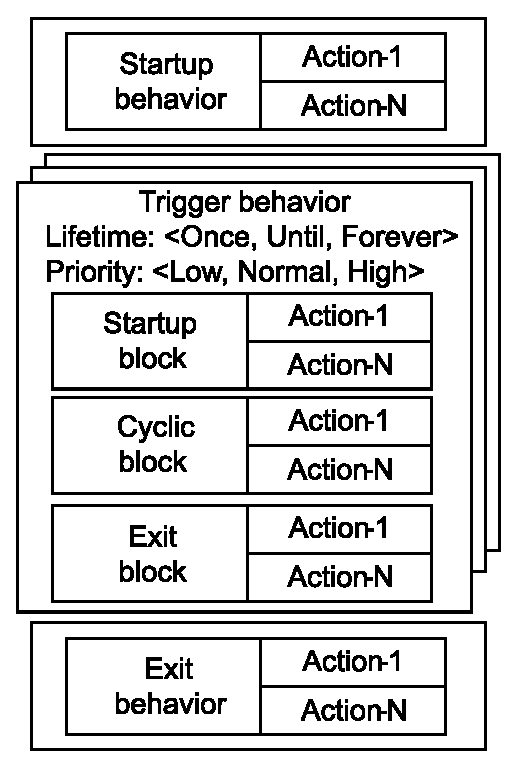
\includegraphics[width=\textwidth]{../thesis/assets/program_structure.eps}
\caption[Conceptual Model]{Conceptual Model}
\label{fig:program_concept}
\end{subfigure}
\begin{subfigure}[t]{0.48\textwidth}
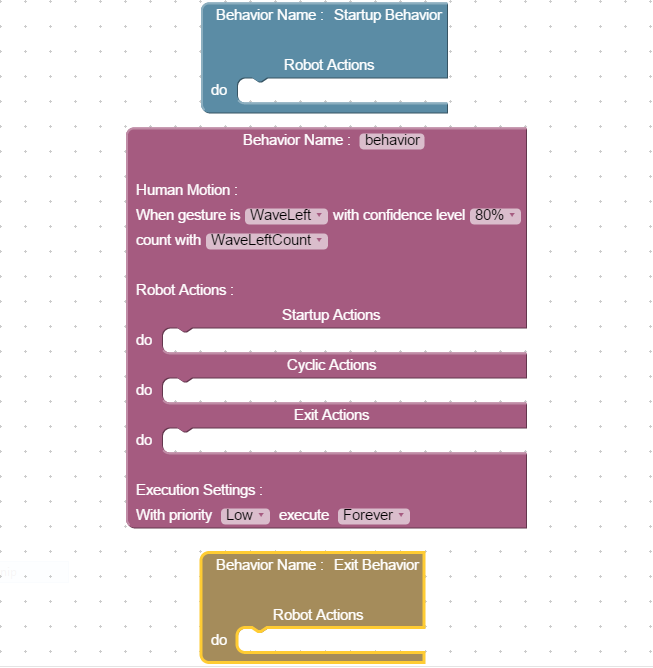
\includegraphics[width=\textwidth]{../thesis/assets/program_block.png}
\caption[Block Implementation]{Block Implementation}
\label{fig:program_blocks}
\end{subfigure}
\caption[Program Structure]{Program Structure}
\label{fig:program}
\end{figure}
The behavior program is structured in a simple way so that it could be easily understood by the end user. The conceptual model of behavior program is shown in Fig.~\ref{fig:program_concept} and the block level implementation is shown in Fig.~\ref{fig:program_blocks}. The behavior program is composed of:
\begin{itemize}
\item \emph{Start-up and Exit Blocks}: The start-up block will be executed once when the user starts the program. The user can add a set of actions to be performed when the program starts. Similarly the exit block will be executed once when the lifetime of all the configured behavior blocks expire.  Both these blocks are optional and there cannot be more than one start-up and exit blocks in a program.
\item \emph{Behavior Block}: The behavior block is composed of
\begin{itemize}
\item A \textbf{trigger} that activates this block. The trigger source could be either of human presence/absence, gesture, vicinity of human, verbal command etc.,
\item The \textbf{lifetime} of each behavior block could be configured to run only once, forever or until a condition is met. 
\item The \textbf{priority} of the block could be set to low, normal or high and the execution is done based on fixed-priority pre-emptive scheduling.
\item Similar to the behavior program level, at each behavior block level a set of \textbf{startup} and \textbf{exit} actions could be set which would be executed only once during the creation and termination respectively. The \textbf{cyclic} actions will be performed each time the trigger condition is met.
\end{itemize}
\end{itemize}
\subsection{Experimental Setup}
\quad The entire framework has been implemented using open network communication standards powered by ZeroMQ \cite{ZeroMQ} and message serialization using the Google's protocol buffers \cite{ProtocolBuffers}. The Kinect for Windows V2 is used as the motion capture system. A set of gestures are created using the visual gesture builder that comes with Kinect SDK \cite{Kinect2014}. The process involves capturing the motion clips, tagging the clips with the appropriate gestures and training the gesture recognizer. The trained gestures are then exported as a visual gesture database and integrated with the motion recognition node. The humanoid robot NAO H25(V50) powered by the latest NaoQi OS V2.1.3 is used for evaluating the interaction scenarios.  A set of actions of the NAO humanoid robot are developed as python scripts. The localization of the humanoid robot is performed by combining the marker detection using augmented reality toolkit ALVAR \cite{ALVAR} and a simple 2-DOF kinematic model of the robot from torso to the head. The software is tested on a 64-bit Intel Core i7 CPU with clock speed 3.60 Ghz and 8 GB of RAM on a Microsoft Windows 8.1 OS. The source code of the software is available as open source at \url{https://github.com/praveenv4k/ICSORO-2015}
\subsection{Example Scenarios}
\begin{figure}
\centering
\begin{subfigure}[t]{0.49\textwidth}
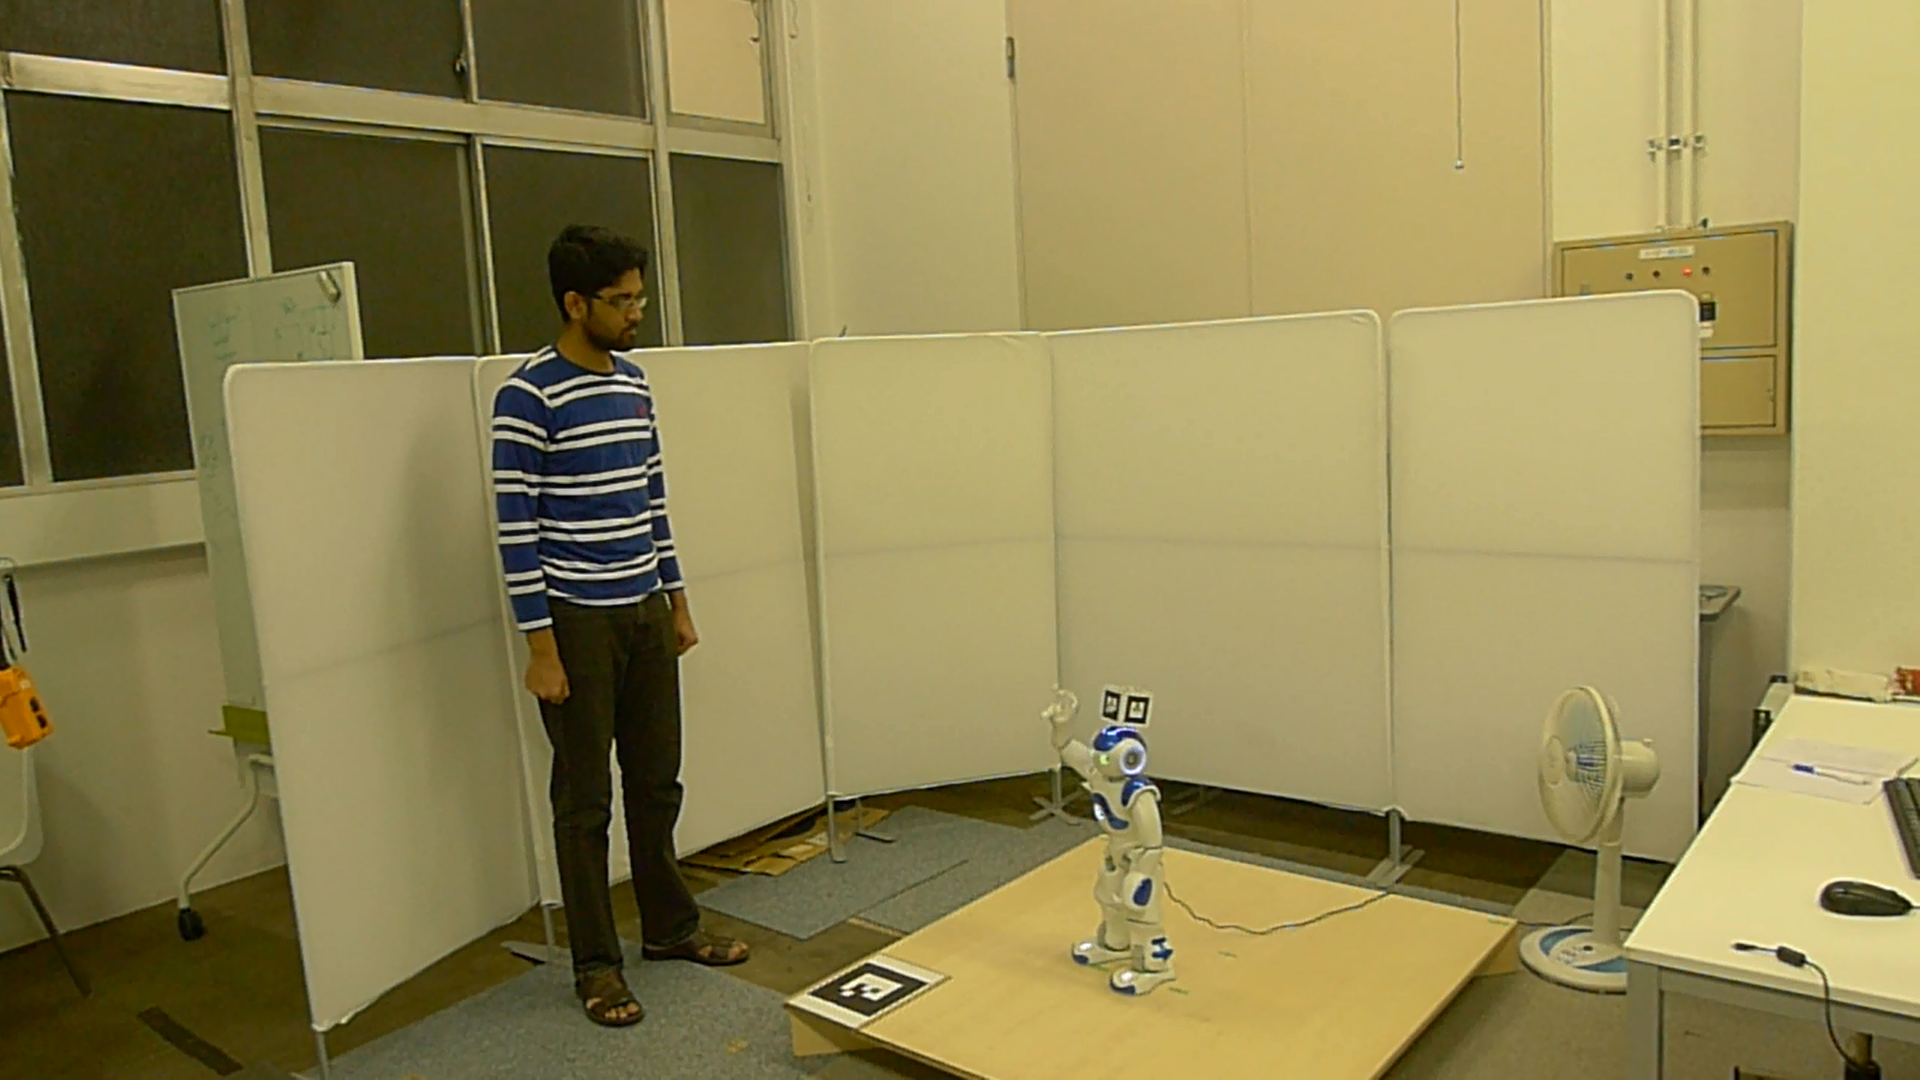
\includegraphics[width=\textwidth]{../thesis/assets/scenario_museum.png}
\caption[Experiment Setup 1]{NAO as demonstrator}
\label{fig:scenario1_setup}
\end{subfigure}
\begin{subfigure}[t]{0.49\textwidth}
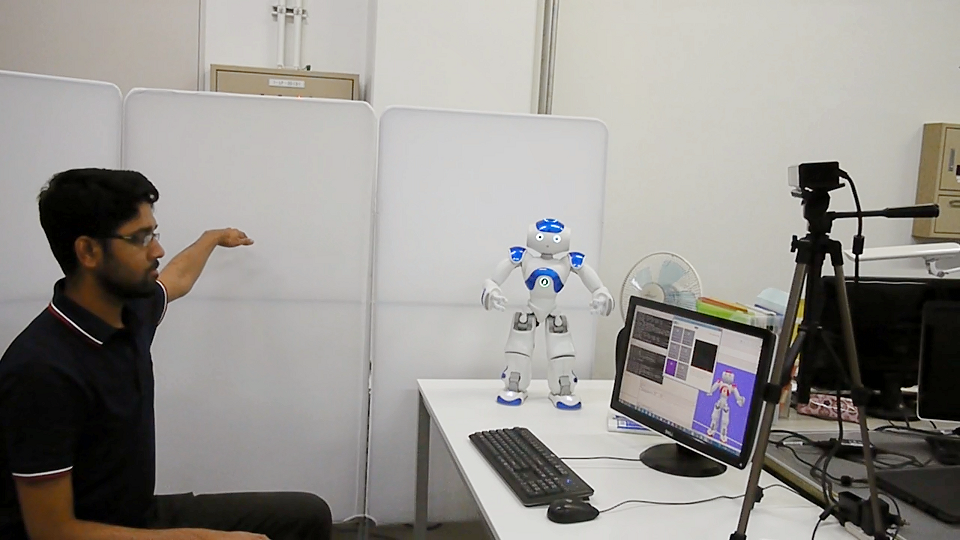
\includegraphics[width=\textwidth]{../thesis/assets/scenario_therapy.png}
\caption[Experiment Setup 2]{NAO therapy facilitator}
\label{fig:scenario2_setup}
\end{subfigure}
\caption[Experiment Setup]{Experiment Setup}
\label{fig:scenarios_setup}
\end{figure}
	In this section we describe two scenarios to demonstrate how our behavior design system could be used for realistic cases which would be otherwise extremely difficult to realize using existing methods for a novice programmer.
\subsubsection{NAO as a demonstrator: }
\begin{figure}
\centering
\begin{subfigure}[t]{0.49\textwidth}
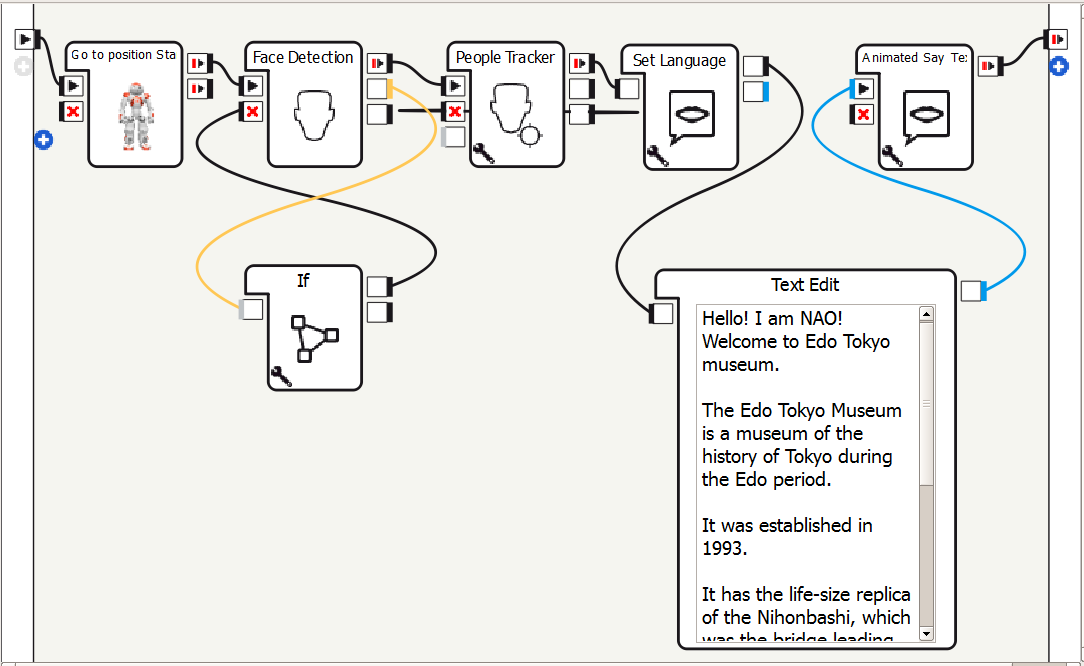
\includegraphics[width=\textwidth]{../thesis/assets/scenario_museum_choregraphe2.png}
\caption[NAO as demonstrator]{Using Choregraphe}
\label{fig:scenario1_program_choregraphe}
\end{subfigure}
\begin{subfigure}[t]{0.49\textwidth}
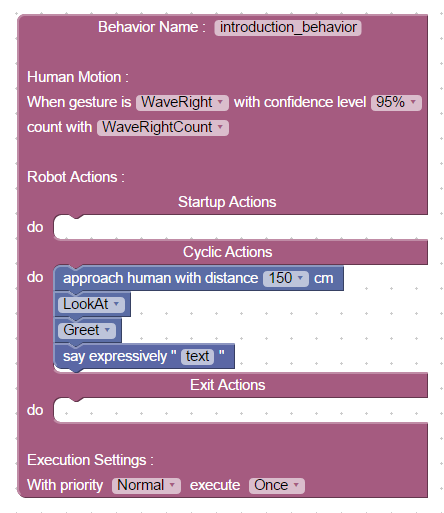
\includegraphics[width=\textwidth]{../thesis/assets/scenario1.png}
\caption[NAO as therapy facilitator]{Using our behavior interface}
\label{fig:scenario1_program}
\end{subfigure}
\caption[NAO as a demonstrator]{NAO as a demonstrator}
\label{fig:scenarios}
\end{figure}
	The NAO humanoid robot is a demonstrator in a museum. The museum manager would like to design a scenario where when a visitor comes into the vicinity of the robot, the robot would approach him/her and start explaining the history of the museum. We would like to use this scenario to compare the expressiveness and intuitiveness of behavior description with Choregraphe \cite{NaoRobot} shown in Fig~\ref{fig:scenario1_program_choregraphe} and with our interface shown in Fig~\ref{fig:scenario1_program}.
	
	Though Choregraphe uses a familiar flow chart based programming model and has a huge library of primitive blocks to build complex motion patterns, the data flow for this scenario is not straight forward. As could be noticed from Fig~\ref{fig:scenario1_program_choregraphe}, at first the robot first keeps looking for people in its vicinity at the cost of its power. Once it detects a person, it stops looking for people and start approaching (tracking) the person until a fixed distance with the person is reached. After this the tracking block has to be stopped and now the robot will actually start explaining the history of the museum.
	
	Using our behavior interface, the definition of this scenario is straightforward as shown in Fig~\ref{fig:scenario1_program}. The framework equipped with Kinect sensor takes care of the detection of people and gives the relative localization of the robot and human. Once the person is detected or a configured gesture trigger arrives, the behavior program retrieves the dynamic position of the robot and of the human. Using this information, the robot is driven towards the person. After coming into the proximity of the person, the robot starts explaining the history of museum. From the user perspective, the design of the behavior is intuitive and he/she can just focus on the scenario rather than thinking about the details of the data flow. The experiment setup for this scenario is shown in Fig~\ref{fig:scenario1_setup}.
\subsubsection{NAO as a therapy facilitator:}%
\begin{figure}
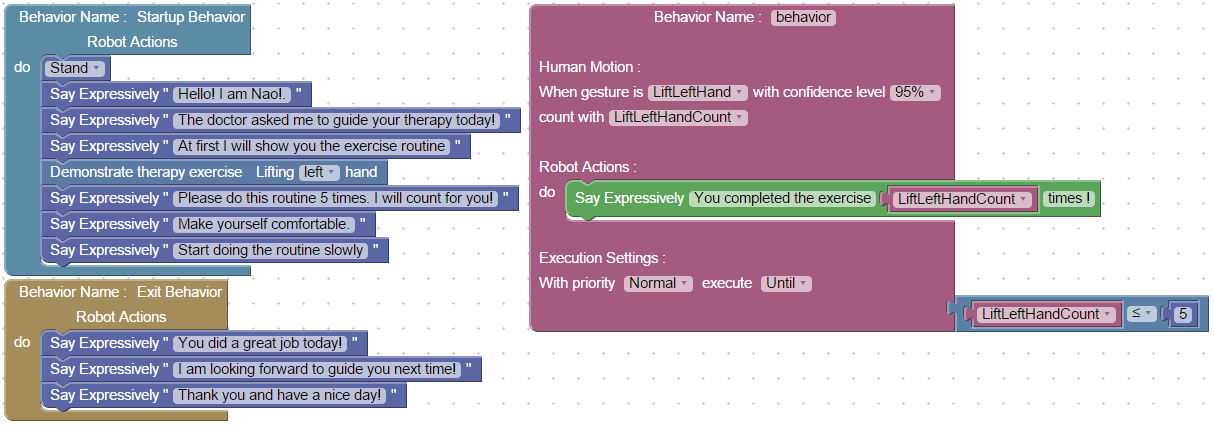
\includegraphics[width=\textwidth]{../thesis/assets/scenario2_horizontal.png}
\caption[NAO as therapy facilitator]{NAO as therapy facilitator}
\label{fig:scenario2_program}
\end{figure}
	A physiotherapist who is in a remote hospital would like to prepare an exercise routine for his patient who is recovering from the fracture of his left hand. The therapist wants the service robot in the rehabilitation center to give directions to the patient in an interactive manner and facilitate the process. The exercise is composed of: an introduction and demonstration of the routine, interactively reporting the progress of the exercise and finally notifying the completion. 
	
	This scenario cannot be realized using choregraphe since it does not explicitly take into account of motion recognition. A reference implementation of such a scenario using our behavior interface is shown in Fig~\ref{fig:scenario2_program}. In the startup behavior an introduction about the exercise routine and a demonstration of the same is performed by the robot. Then each time the patient performs the exercise, the robot notifies the progress of the exercise. Once the exercise routine is completed (say lifting left hand 5 times), the robot gives some closing comments about the routine. The experiment setup for this scenario is shown in Fig~\ref{fig:scenario2_setup}.
\section{Conclusion}
\quad The abundance of smart devices and sensors in the smart home and public environments provide rich information about the human motions. This information could be used for an immersive and personalized human robot interaction experience. The people from interdisciplinary fields wanting to develop a rich interaction scenario find it difficult to use the existing technology as it requires strong background in programming. Any new programming paradigm designed for such purposes should find a correct balance between simplicity and expressiveness which was the main motivation behind our proposal. We believe that our proposal could be used for studying various aspects of HRI such as efficiency of the system, cooperativeness, social acceptance etc., There exist some open questions and challenges to be addressed however. The preliminary challenges are to find a set of all possible human motions that could be understood from the sensors distributed around in the environment and to identify all possible actions a robot could perform to interact with human in a social interaction scenario. The next question is to find the spectrum of interaction scenarios this kind of programming interface could cover. It is also extremely important to evaluate the usability of the system by making statistical analysis collected on a set of participants and naive users.
\section{Prospective work}
\quad This is a work in progress and for the moment we have evaluated our system for the Kinect motion capture system working seamlessly with the NAO humanoid robot for a set of predefined gestures and robot actions. We are planning to develop an extensive database containing commonly encountered gestures and also an extensive set of primitive robot actions. Additionally we are also planning to integrate our system to work with other modes of motion recognition like inertial measurement units (IMU), accelerometers and gyroscopes that are available in smart-phones and wearable devices. Similarly we are planning to integrate our system with other robots like Turtlebot and Pepper which we expect to receive soon.
\section{Acknowledgments}
		We would like to thank the members of GVLab at Tokyo University of Agriculture and Technology for helping us arranging the resources and participating in the experimentation. This work has been supported by Student Exchange Support Program of Japan Student Services Organization (JASSO).
\bibliographystyle{plain}
\bibliography{../Thesis/Bibliography}
\end{document}
